\section{Conclusion and Work Plan}
\label{sec:conclusion}
The pilot work just described is exciting and compelling, and it demonstrates the value of our proposed work. First, we are able to verify the most comprehensive model of discrimination and its impact on behavior and outcomes to date. As illustrated in Figure~\ref{fig:model}, we hypothesize that discrimination's impact on mental and physical health will affect those stress-related behaviors (\ref{itm:rq-behavior}). Our study will not only help to test that hypothesis but also to quantify the scope, direction, and longitudinal impact of discrimination on each type of behavior, improving our theoretical model of discrimination's impact on individuals (\ref{itm:rq-behavior-size}, \ref{itm:rq-severity-impact}).
 
 In addition, ours is the first model at this level of detail to tie discrimination specifically to student outcomes, such as GPA and retention. Our model will help to link short-term behavior to long-term outcomes (\ref{itm:rq-short-long}, \ref{itm:rq-which-long}, \ref{itm:rq-which-long}). This makes it extremely valuable for helping with intervention design and policy setting on university campuses.
 For example, the buffering effect of social support has implications for intervention design. 

Lastly, our approach is the first to explore the relationship between specific micro-climates and the mediating factors that help to buffer people from the impact of discrimination (\ref{itm:mc-daily-discrimination}, \ref{itm:mc-internal-mediators}, \ref{itm:mc-external-mediators}). By studying micro-climate impact on outcomes, we can further support intervention design and enrich our theoretical model. 

Educational institutions are characterized by dominant attitudes and behaviors. Some disciplines are particularly vulnerable to gender, race, and nationality bias, including  engineering \cite{sevo2010bias}.  We believe that it is critically important to study these issues in the educational context, a sentiment recently argued in an NSF Dear Colleague Letter encouraging research in sexual harassment and other forms or harassment in STEM contexts.\footnote{\url{www.nsf.gov/pubs/2019/nsf19053/}} The pervasiveness of discrimination experiences in our data surprised even our seasoned team, and addressing them is critical to creating a diverse and informed workforce. This can be accomplished only by shedding light on these darker aspects of engineering education. As Bill and Melinda Gates said in their  recent Annual Letter,\footnote{\url{https://www.gatesnotes.com/2019-Annual-Letter}} data is sexist (and racist), and the biases inherent in the data we collect are necessary, indeed critical, to address. This study is a first attempt to do so, and we intend to contribute to the development of this domain as an important topic of study for computational researchers.   

%A comprehensive change in the way that we study the college student experience. 
%Our research facilitates this thanks to new changes in the ease of capturing real-time student information. Our work is innovative because it allows us to study the student experience at scale, provides before-after data around events such as discrimination,
% quantifies impact, and allow us to design the most effective interventions and policies.
 
Our work plan is as follows: 


%\begin{table}[]
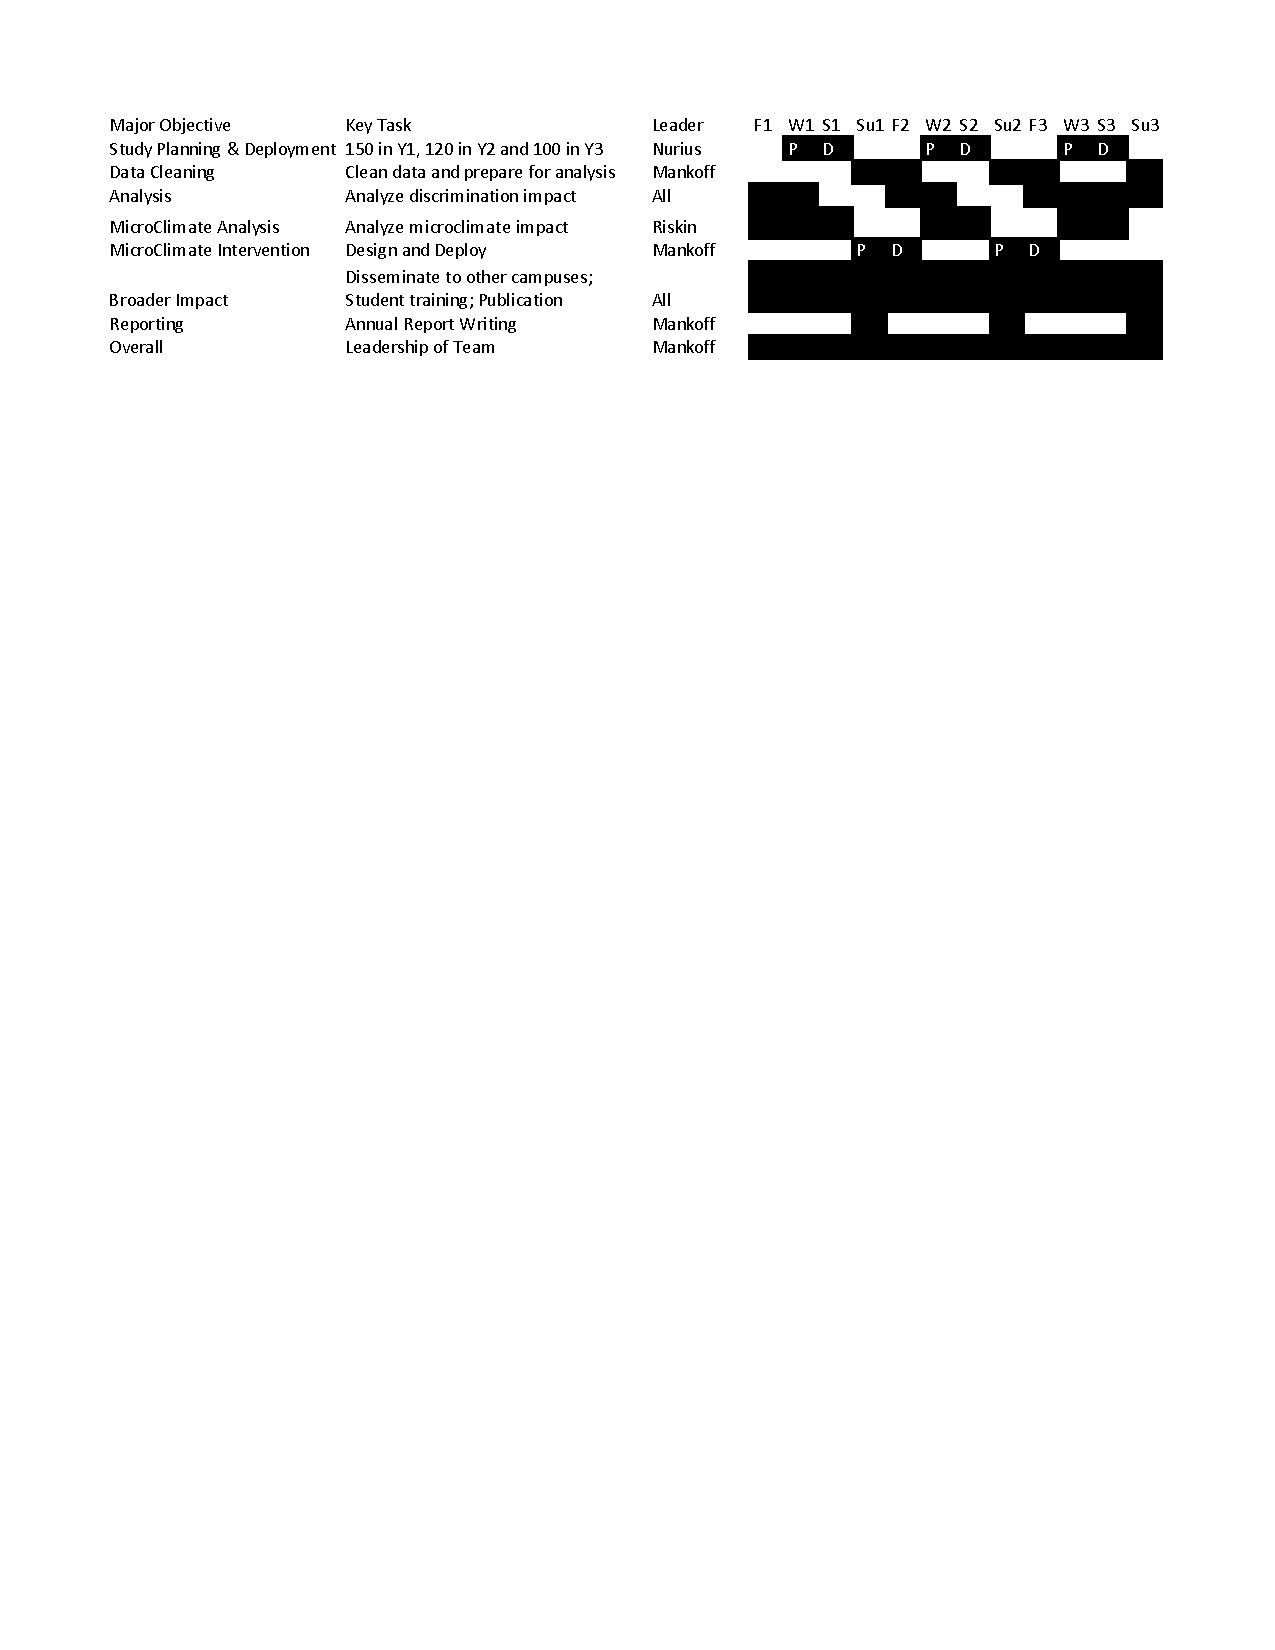
\includegraphics[width=\textwidth]{img/workplan.pdf}
% \small
% \resizebox{\textwidth}{
% \begin{tabular}{p{3cm}p{3cm}lllllllllllll}
% \textbf{Major Objective} &  \textbf{Key Task} & \textbf{Leader} &  F1 &  W1 & S1 & Su1 & F2 & W2 & S2 & Su2 & F3 & W3 & S3 & Su3 \\ \hline
% Study Planning \& Deployment & 150 in Y1, 120 in Y2 and 100 in Y3 & Nurius &  &  P &  D &  &  &  P & D &  &  & P & D &  \\
% Data Cleaning & Clean data and prepare for analysis & Mankoff &  &  &  & X & X &  & X & X &X &  &  & X \\
% Analysis & Analyze discrimination impact & All & X&X&  &  &X& X  &  &  & X & X & X & X\\
% Microclimate Analysis & Analyze microclimate impact & Riskin &X&X & X &  &  & X & X &  &  &X&X &  \\
% Microclimate Intervention & Design and deploy & Mankoff &  &  &  & P & D &  &  &  P &  D &  &  &  \\
% Broader Impact & \begin{tabular}[c]{@{}l@{}}Disseminate to other campuses; \\ Student training; publication\end{tabular} & All &  & X & X & X & X & X & X & X & X & X& X& X& X\\
% Reporting & Annual Report writing & Mankoff &  &  &  & X &  &  &  & X &  &  &  & X \\
% Overall & Team leadership & Mankoff & X & X & X & X & X & X & X & X & X& X& X& X
% \end{tabular}%
% }
%\end{table}

\subsection{Risks and Limitations}
While this study represents a major undertaking, and our pilot data and analysis provide promising evidence of the potential for this data set to shed light on important problems, there are always risks that must be considered. Here we address a few:

The duration of our study may be short for substantial changes in health 
due to the events happening during the study to fully develop. Nonetheless, we expect to observe differences because it is likely that people who reported being unfairly treated in our study have had other experiences in the past that have adversely changed their mental health status with identifiable behavior signals.   

Additionally, this proposal is limited specifically to discrimination. There are many other traumatic events (such as sexual harrassment) that students might encounter, but discrimination is unique in how common and prevalent it is according to our data and thus well suited to the proposed work.

Finally, although we study micro-climates, this proposal does not include novel interventions, nor does it control directly who benefits from those micro-climates and who does not. Given our sample sizes, this limits the degree to which we can draw clear causal lines. However, we expect our proposed work to help provide new perspectives on what sorts of interventions are worth developing and lead to such developments in the future. 